\documentclass[10pt]{article}
\usepackage[margin=2cm]{geometry}
\usepackage{amsmath,amssymb}
\usepackage{booktabs,multirow,array}
\usepackage{graphicx}
\usepackage{caption}
\usepackage[hidelinks]{hyperref}
\captionsetup{font=small,labelfont=bf}
\makeatletter\let\inputrows\@@input\makeatother
\setlength{\parskip}{3pt}\setlength{\parindent}{0pt}

\title{\textbf{CT-KAE candidates on Kuramoto--Sivashinsky}}
\date{1 November 2026}
\author{}

\begin{document}
\maketitle
\vspace{-2.5em}

\section*{Summary}
The two transonic CT-KAE candidates (the reference and back001) were trained on KS with the transonic
recipe and run through every KS experiment of the paper. The paper's KAE, U-Net and SDA are the
baselines.
\begin{itemize}\itemsep1pt
\item \textbf{Forecasting fails beyond one training horizon.} The CT-KAEs have the best
  encode--decode accuracy of the four models (0.007), but their error grows ten-fold every ten steps.
  At $0.1\,T_L$ it is 0.58--0.64, against 0.024 for the paper's KAE and 0.0003 for the U-Net. Skill is
  lost at 0.3--0.4 $T_L$ (paper's KAE 2.4, U-Net 9.3).
\item \textbf{DA is close to the paper's KAE when the first observation is close to $t_0$.} The
  canonical analysis is 0.025--0.028 (paper's KAE 0.0044, SDA 0.009, U-Net 0.097). The CT-KAEs match
  the paper's KAE with $\ge 13$ observation times. They are the best of all five models with 25--50\%
  sensor coverage and many observation times.
\item \textbf{DA is worse than the paper's KAE} when the first observation is later than 0.1 t.u., with
  noise (3--6$\times$), and in long windows.
\item \textbf{Of the transonic readouts, only the sharpened symmetry average is admissible on KS.} It
  halves the 50-frame error, to just under persistence. LPM fails.
\item \textbf{back001 vs the reference:} back001 has a slightly longer forecast skill, within seed
  spread; DA is the same.
\item \textbf{The cause is not established.} It is not the rollout length alone: the paper's KAE
  also trains on 10-frame windows and keeps skill for 2.4 $T_L$. The largest difference is the
  training budget. The transonic recipe (batch 16, 20k steps) shows the CT-KAE 0.3M windows; the
  paper's KAE saw $\sim$16M (batch 1024, 200 epochs over all 79k windows of \texttt{train.nc}). A
  CT-KAE retrained at the paper's budget would test this.
\end{itemize}

\section*{Setup}
\begin{itemize}\itemsep1pt
\item \textbf{Models.} The two transonic candidates, the reference and back001 (the reference plus
  backward latent consistency at weight 0.01), trained on KS with the transonic recipe: latent
  dimension 256, widths 64/128/256, 128 damped oscillators (exact $e^{\tau A}$), no fixed point,
  reconstruction + 8-lead prediction + latent consistency + amplitude terms, 20k steps, batch 16,
  AdamW $3\times10^{-4}$, final checkpoint, 3 seeds each. KS-specific changes: 1-D convolutions with
  circular padding, one input frame (KS is Markovian; the paper's KS models also encode one frame),
  no physical parameter, $\Delta t = 0.1$ (the transonic step). Training: \texttt{train.nc} (80
  trajectories); \texttt{val.nc} only logged. About 8 minutes per run on one RTX 4090.
\item \textbf{Baselines.} The paper's KS KAE, U-Net and SDA. Their numbers are the paper's stored
  results on the same seeded problems. The paper's KAE cannot be re-run: with today's code its
  encode--decode error is 0.135 instead of the 0.009 recorded in August (identical architecture,
  strict checkpoint load; the forward pass probably changed in the September refactor).
\item \textbf{Protocol.} The paper's KS code, unmodified, with the CT-KAE in the KAE slot
  (\texttt{audit\_report/\allowbreak scripts/\allowbreak ks\_ctkae/\allowbreak ks\_driver.py}). Two adaptations, both decided on
  validation data: (i) the 4D-Var control is the latent normalised per dimension by its
  training-split standard deviation (an exact change of variables: the CT-KAE latents have a
  scale of $\sim$350, the paper's KAE $\sim$1, for which the learning-rate grid was built);
  (ii) the initialisation grid adds the harness's informed first guess $e^{-A\tau_1}E(y_1)$ to
  \{random, zero\}. Validation selected the informed first guess and learning rate 0.03 for both
  candidates (validation error 0.231 and 0.226; the paper's KAE 0.189 with zero start); from zero,
  the CT-KAE does not leave the latent origin's basin (validation error $\approx1$). DA results are
  for seed 0.
\end{itemize}

\section*{Forecasting}
\begin{table}[!htbp]
\centering\scriptsize
\caption{Free-running forecast from the true state (\texttt{da\_test\_long}, 32 trajectories,
$T_L = 22.6$ t.u.): relative $L_2$ error at leads in Lyapunov times, the skill horizon (error
reaching 90\% of the no-skill level) and the encode--decode error at $t_0$. CT-KAE: mean $\pm$ SE
over 3 seeds.}
\label{tab:ksfc}
\resizebox{\linewidth}{!}{%
\begin{tabular}{lcccccc}
\toprule
 & $0.1\,T_L$ & $0.5\,T_L$ & $1\,T_L$ & $5\,T_L$ & skill horizon ($T_L$) & round trip\\
\midrule
\inputrows tab_ks_forecast.tex
\bottomrule
\end{tabular}}
\end{table}

The CT-KAEs are the most accurate models of the four over a few steps and the least accurate beyond
one training horizon. Their encode--decode error (0.007--0.008) is below the paper's KAE (0.017 in
this file, 0.009 in the paper's AE audit), and their one-step error on \texttt{test.nc} is 0.008. But
the error grows ten-fold every ten steps (0.089 at 1 t.u., 0.51 at 2.2 t.u.; seed 0 reference), so at
$0.1\,T_L$ it is already 0.58--0.64 against 0.024 for the paper's KAE and 0.0003 for the U-Net, and skill
is lost at 0.28--0.38 $T_L$ (paper KAE 2.4, U-Net 9.3). This growth is model error, not chaos: the
learned generators are strictly stable (largest real part $-0.0075$ to $-0.0088$ over six runs; the
leading Lyapunov exponent is $+0.044$). Training rolls out 8 steps (0.8 t.u.), which is roughly where the error leaves the
encode--decode floor; the paper's KAE trains on 10 frames, so the rollout length alone does not
explain the gap (see the summary). back001 is ahead at short leads (0.575 vs 0.643 at
$0.1\,T_L$; horizon 0.38 vs 0.28 $T_L$), with seed spread of the same order.

\begin{figure}[!htbp]
\centering
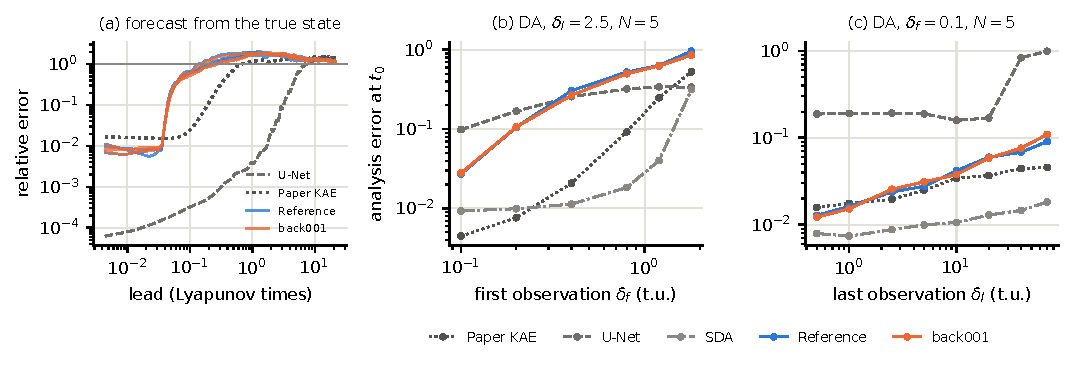
\includegraphics[width=\linewidth]{fig_ks.pdf}
\caption{(a) Forecast error from the true state (CT-KAE: 3 seeds each). (b, c) Analysis error of
4D-Var against the lead of the first and of the last observation (48 and 24 problems; CT-KAE:
seed 0).}
\label{fig:ks}
\end{figure}

\section*{Data assimilation}
\begin{table}[!htbp]
\centering\scriptsize
\caption{Analysis error at $t_0$ (relative $L_2$, mean over 48 problems; 24 for $\delta_l$) of
every sweep of the paper, on the same problems. Defaults: $\delta_f = 0.1$, $\delta_l = 2.5$
t.u., $N = 5$, full coverage, no noise; 8000 iterations (1000 for $\delta_l$). Best per row in
bold. $N$ is the realised number of observation times (rounding to the frame grid drops
duplicates).}
\label{tab:ksda}
\begin{tabular}{lccccc}
\toprule
 & Paper KAE & U-Net & SDA & Reference & back001\\
\midrule
\inputrows tab_ks_da.tex
\bottomrule
\end{tabular}
\end{table}

When the first observation is one step after $t_0$ (the paper's campaign), the CT-KAEs are DA
models of the same class as the paper's KAE, ahead of the U-Net except at noise $\sigma \ge 0.2$,
and ahead of SDA in places:
\begin{itemize}\itemsep1pt
\item \textbf{Canonical window} ($N = 5$): 0.025--0.028, against 0.0044 for the paper's KAE, 0.009 for
  SDA and 0.097 for the U-Net.
\item \textbf{More observation times close this gap.} With 8 times the error is 0.009, and with 13
  or 16 it is 0.006, level with the paper's KAE (0.0055--0.0060).
\item \textbf{Sparse sensors with many times} are the CT-KAEs' best regime. At 25\% coverage with
  8 or 13 times they are the best of the five (0.014--0.019, against 0.070 for the paper's KAE and
  0.018--0.021 for SDA). At 50\% coverage with 13 times they are also best (0.008 against 0.010 for SDA).
\item \textbf{Short windows} ($\delta_l \le 1$ t.u., 1000 iterations): 0.012--0.016, slightly better
  than the paper's KAE (0.016--0.018).
\item \textbf{The first observation must be close to $t_0$.} The error grows to 0.11 at
  $\delta_f = 0.2$ and 0.27--0.31 at $\delta_f = 0.4$ (paper's KAE 0.008 and 0.021). This follows from the
  forecast error: inverting the model over $\delta_f$ costs what forecasting over $\delta_f$ costs.
  The main repository's $\delta_f = 0.9$ campaign (Table~\ref{tab:ksda9}) shows the same: about 0.5 at
  $N = 5$, against 0.12 for the paper's KAE and 0.02 for SDA.
\item \textbf{Noise is the weakest regime}: 3--6$\times$ the paper's KAE at every level
  ($\sigma = 0.05$: 0.11--0.12 against 0.034; $\sigma = 0.4$: 0.90--0.97 against 0.24--0.26).
\item \textbf{Long windows}: on \texttt{da\_test\_long} the error rises from 0.024--0.026 at
  $0.11\,T_L$ to 0.09--0.13 at $17.7\,T_L$ (paper's KAE 0.018 to 0.073). In the $\delta_l$ sweep it
  rises from 0.024--0.026 at 2.5 t.u. to 0.09--0.11 at 70 t.u. (paper's KAE 0.046, SDA 0.018).
\item \textbf{Forecast from the analysis} (Table~\ref{tab:kspf}): the analysis is good (0.036--0.037,
  paper's KAE 0.013), but the forecast from it inherits the propagator. Skill is lost at
  0.34--0.40 $T_L$, against 0.53 for the paper's KAE and 10.9 for the U-Net. The U-Net's analysis error
  (0.147) is in modes that decay within a few steps; its forecast error at $0.1\,T_L$ is $10^{-4}$.
\end{itemize}
The two candidates are within seed-level differences of each other throughout. back001 is not
reliably better in DA.

\begin{table}[!htbp]
\centering\scriptsize
\caption{The same sweeps with the first observation at $\delta_f = 0.9$ t.u. (the main repository's
\texttt{da\_results\_geometry\_df9} campaign, the current default of \texttt{exp\_geometry}; same
schedules frame for frame). Defaults: $\delta_l = 2.5$ t.u., $N = 5$, 8000 iterations (1000 for
$\delta_l$).}
\label{tab:ksda9}
\begin{tabular}{lccccc}
\toprule
 & Paper KAE & U-Net & SDA & Reference & back001\\
\midrule
\inputrows tab_ks_da9.tex
\bottomrule
\end{tabular}
\end{table}

\begin{table}[!htbp]
\centering\scriptsize
\begin{minipage}[t]{0.52\linewidth}\centering
\caption{Long-baseline assimilation (\texttt{da\_test\_long}; $\delta_f = 0.1$, $N = 5$, 1000
iterations, 24 problems). U-Net and SDA are capped by cost.}
\label{tab:kslb}
\begin{tabular}{ccccccc}
\toprule
$\delta_l$ & $T_L$ & Paper KAE & U-Net & SDA & Ref. & back001\\
\midrule
\inputrows tab_ks_lb.tex
\bottomrule
\end{tabular}
\end{minipage}\hfill
\begin{minipage}[t]{0.45\linewidth}\centering
\caption{Forecast from each method's own analysis (canonical window, 24 problems, 2000
iterations).}
\label{tab:kspf}
\begin{tabular}{lcccc}
\toprule
 & analysis & $0.1\,T_L$ & $1\,T_L$ & horizon ($T_L$)\\
\midrule
\inputrows tab_ks_postda.tex
\bottomrule
\end{tabular}
\end{minipage}
\end{table}

\begin{figure}[!htbp]
\centering
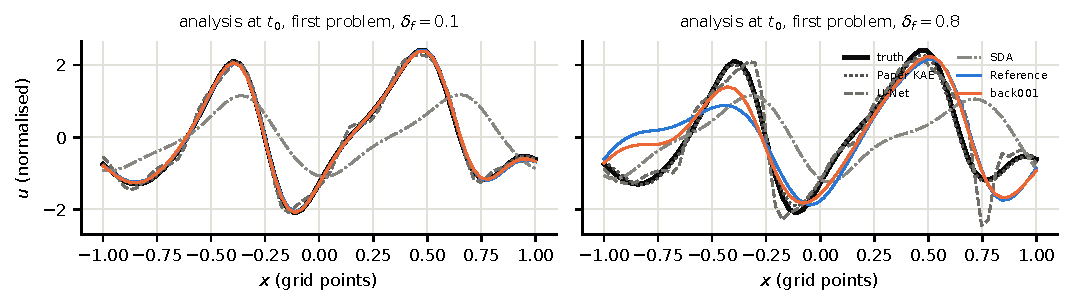
\includegraphics[width=\linewidth]{fig_ks_fields.pdf}
\caption{Analyses at $t_0$ of the first problem of the $\delta_f$ sweep, against the truth.}
\label{fig:ksfields}
\end{figure}

\section*{Post-processing readouts on KS}
\begin{table}[!htbp]
\centering\scriptsize
\caption{The transonic readouts on the CT-KAE's KS forecasts (\texttt{test.nc}, from the true
state; short: 50 frames from 10 starts per trajectory, long: 400 frames from 3). MSE (normalised)
of the single decode, then MSE relative to it (mean $\pm$ SE over 3 seeds), and the $\log_{10}$
power ratio prediction / truth at low ($k \le 3$) and high ($k = 7$--$10$) wavenumbers. KS is
symmetric under periodic shifts and $u(x) \to -u(-x)$; both give members.}
\label{tab:kspp}
\begin{tabular}{llcccccc}
\toprule
 & & \multicolumn{3}{c}{short} & \multicolumn{3}{c}{long}\\
\cmidrule(lr){3-5}\cmidrule(lr){6-8}
 & & MSE & low & high & MSE & low & high\\
\midrule
\inputrows tab_ks_pp.tex
\bottomrule
\end{tabular}
\end{table}

The readouts cannot repair forecasts this far off. Over 50 frames the single decode (MSE 0.48 /
0.39) is worse than persistence (0.29); the U-Net is at $5\times10^{-8}$. On KS the symmetries play
the role of the transonic mirror average: averaging the decodes of the 4 shifted $\times$ 2
reflected encodings lowers MSE by a factor of 0.54--0.65 (short) and 0.34--0.37 (long). But at long
leads it removes most of the low-wavenumber power ($\log_{10}$ ratio $-1.1$): the drop comes from
regressing towards the climatological mean, which is blurring. Sharpening keeps most of the gain
at short leads (0.50--0.61) and restores power at low $k$ ($-0.4$), with too much power at high $k$
at long leads. LPM, the best transonic readout, fails here: with 64 points a 16-point patch is a
quarter of the domain, and the patch-wise rank matching adds 30--300$\times$ power at $k = 7$--10. On
KS, the sharpened symmetry average is the only admissible readout; it brings the 50-frame error
(0.24 for both candidates) just under persistence.

\end{document}
